% !TeX TXS-program:compile = txs:///arara
% arara: pdflatex: {shell: yes, synctex: no, interaction: batchmode}
% arara: pdflatex: {shell: yes, synctex: no, interaction: batchmode} if found('log', '(undefined references|Please rerun|Rerun to get)')

\documentclass[french,11pt,a4paper]{article}
\usepackage[utf8]{inputenc}
\usepackage[T1]{fontenc}
\RequirePackage[upright]{fourier}
\RequirePackage{mathtools}
\RequirePackage{amsmath,amssymb,amstext}
\RequirePackage[scaled=0.875]{helvet}
\renewcommand\ttdefault{lmtt}
\RequirePackage[scaled=0.925]{cabin} % sf
%\usepackage{DejaVuSerif}
%\usepackage[scale=1.1]{inconsolata}
\usepackage{customenvs}
\usepackage{tabularx}
\usepackage{soul}
%\usepackage{codehigh}
\usepackage{fontawesome5}
\usepackage{lipsum}
\usepackage{fancyvrb}
\usepackage{fancyhdr}
\fancyhf{}
\renewcommand{\headrulewidth}{0pt}
\lfoot{\sffamily\small [customenvs]}
\cfoot{\sffamily\small - \thepage{} -}
\rfoot{\hyperlink{matoc}{\small\faArrowAltCircleUp[regular]}}
\usepackage{hologo}
\providecommand\tikzlogo{Ti\textit{k}Z}
\providecommand\TeXLive{\TeX{}Live\xspace}
\providecommand\PSTricks{\textsf{PSTricks}\xspace}
\let\pstricks\PSTricks
\let\TikZ\tikzlogo

\usepackage{hyperref}
\urlstyle{same}
\hypersetup{pdfborder=0 0 0}
\usepackage[margin=1.5cm]{geometry}
\setlength{\parindent}{0pt}

\def\TPversion{0.1.3}
\def\TPdate{30 mars 2024}
\usepackage[most]{tcolorbox}
\tcbuselibrary{listingsutf8}
\newtcblisting{DemoCode}[1]{%
	enhanced,width=0.95\linewidth,center,%
	bicolor,size=title,%
	colback=cyan!5!white,%
	colbacklower=cyan!1!white,%
	colframe=cyan!75!black,%
	listing options={%
		breaklines=true,%
		breakatwhitespace=true,%
		style=tcblatex,basicstyle=\small\ttfamily,%
		tabsize=4,%
		commentstyle={\itshape\color{gray}},
		keywordstyle={\color{blue}},%
		classoffset=0,%
		keywords={usepackage,displaystyle,frac,infty,begin,end,lipsum,centering,par,baselineskip,item,bullet,int,color,NewDocumentCommand},%
		alsoletter={-},%
		keywordstyle={\color{blue}},%
		classoffset=1,%
		alsoletter={-},%
		morekeywords={center,justify,\LstDeuxNiv,\LstTroisNiv,\LstQuatreNiv,\NoticeDeuxNiv,\NoticeTroisNiv,\NoticeQuatreNiv,\DeuxNivBatterie,\TroisNivBatterie,\QuatreNivBatterie,\DeuxNivSmiley,\TroisNivSmiley,\QuatreNivSmiley,\vcenterfa,\faIcon},%
		keywordstyle={\color{violet}},%
		classoffset=2,%
		alsoletter={-},%
		morekeywords={\ReponsesQCM,MultiCols,\CreerListeItems,\ListeChoixItems,\TableauCompetences,\CrayonDeCompetences,\StyleEnvtExo,\StyleEnvtExoDefaut,\TitreExo,\ipsum},%
		keywordstyle={\color{green!50!black}},%
		classoffset=3,%
		morekeywords={Largeur,Filets,EspacesCL,NbCols,Labels,PoliceLabels,EspaceLabels,Swap,Type,CoeffEspVert,EpTrait,Alea,LargeurNivs,Niveaux,NoticeNiveaux,Titre,PolTitre,PolNotice,PolComp,LigneSep,CouleurNotice,CouleurNiveaux,CouleurFond,Note,Notice,PoliceCateg,PoliceBloc,Couleurs,LargeurBloc,Echelle,NoirBlanc,Libelle,EpTrait,Police,Type,ComplementTitre,Titre,CodeDebut,Couleur,EchelleImage,Decoration,Trait},%
		keywordstyle={\color{orange}}
	},%
	#1
}
\sethlcolor{lightgray!25}
\NewDocumentCommand\MontreCode{ m }{%
	\hl{\vphantom{\texttt{pf}}\texttt{#1}}%
}

\usepackage{babel}

\begin{document}

\pagestyle{fancy}

\thispagestyle{empty}

\begin{center}
	\begin{minipage}{0.75\linewidth}
	\begin{tcolorbox}[colframe=yellow,colback=yellow!15]
		\begin{center}
			\renewcommand\arraystretch{1.25}
			\begin{tabular}{c}
				{\Huge \texttt{customenvs [fr]}}\\
				\\
				{\Large Quelques environnements classiques,} \\
				{\Large légèrement modifiés, et basés} \\
				{\Large sur des environnements existants.} \\
			\end{tabular}
			\renewcommand\arraystretch{1}
			
			\medskip
			
			{\small \texttt{Version \TPversion{} -- \TPdate}}
		\end{center}
	\end{tcolorbox}
\end{minipage}
\end{center}

\vspace*{1mm}

\begin{center}
	\begin{tabular}{c}
	\texttt{Cédric Pierquet}\\
	{\ttfamily c pierquet -- at -- outlook . fr}\\
	\texttt{\url{https://github.com/cpierquet/customenvs}}
\end{tabular}
\end{center}

\vspace*{5mm}

%\hrule
%
%\vspace*{2mm}
%
%{\centering Le nom du package vient de \textsf{ENVironnemenTS ALTernatifs}, avec le suffixe \textsf{FRançais}.\par}
%
%\vspace*{2mm}
%
%\hrule
%
%\vspace*{1cm}

\hrule

\phantomsection

\hypertarget{matoc}{}

\tableofcontents

\vspace*{5mm}

\hrule

\pagebreak

\section{Historique}

\verb|v0.1.3|~:~~~~Environnement/commande pour des exercices, avec personnalisation(s)

\verb|v0.1.2|~:~~~~Crayon de compétences

\verb|v0.1.1|~:~~~~Tableaux de compétences

\verb|v0.1.0|~:~~~~Version initiale

\pagebreak

\section{Le package customenvs}

\subsection{Idée}

L'idée est de proposer des commandes ou environnements classiques avec quelques éléments de personnalisation (via des \textsf{clés} francisées), comme :

\begin{itemize}
	%\item modifier localement l'\textit{alignement vertical} d'éléments sans jambage ;
	\item \textit{centrer} avec gestion des espacements autour ;
	\item écrire en \textit{multi-colonnes} avec gestion des espacements autour ;
	\item mettre en forme des réponses à des \textit{QCM} ;
	\item créer une liste avec \textit{choix des items} (de manière aléatoire ou par saisie directe) ;
	\item créer un tableau de \textit{compétences}.
\end{itemize}

\smallskip

L'idée globale est de proposer des environnements clé en main, avec personnalisations \textit{explicites}, sans forcément avoir besoin de \textit{se pencher sur le code}, mais il est évident qu'il existe d'autres solutions pour l'utilisateur qui souhaite réellement contrôler son rendu.

\smallskip

Il est ici essentiellement question de gérer les espacements, donc on peut citer comme autres solutions possibles :

\begin{itemize}
	\item l'utilisation de \MontreCode{\textbackslash vspace} ou de \MontreCode{\textbackslash  setlength} ;
	\item le package \MontreCode{spacingtricks}.
\end{itemize}

\subsection{Chargement}

Le package se charge dans le préambule, via \MontreCode{\textbackslash usepackage\{customenvs\}}.

Les packages chargés sont :

\begin{itemize}
	\item \MontreCode{xstring}, \MontreCode{simplekv}, \MontreCode{listofitems}, \MontreCode{randomlist} et \MontreCode{xintexpr} ;
	\item \MontreCode{enumitem} ;
	\item \MontreCode{multicol} ;
	\item \MontreCode{tabularray} ;
	\item \MontreCode{xcolor} ;
	\item \MontreCode{fontawesome5}.
\end{itemize}

À noter que, pour des raisons de compatibilité (ou d'incompatibilité), les packages \MontreCode{enumitem}/\MontreCode{multicol}/\MontreCode{tabularray}/\MontreCode{xcolor}/\MontreCode{fontawesome5} peuvent ne pas être chargés par \MontreCode{customenvs} (auxquels cas l'utilisateur devra les avoir chargés pour faire fonctionner certains environnements) via les options :

\begin{itemize}
	\item \MontreCode{$\mathtt{\langle}$nonenum$\mathtt{\rangle}$} ;
	\item \MontreCode{$\mathtt{\langle}$nonmulticol$\mathtt{\rangle}$} ;
	\item \MontreCode{$\mathtt{\langle}$nontblr$\mathtt{\rangle}$} ;
	\item \MontreCode{$\mathtt{\langle}$nonxcolor$\mathtt{\rangle}$} ;
	\item \MontreCode{$\mathtt{\langle}$nonfa$\mathtt{\rangle}$}.
\end{itemize}

\begin{DemoCode}{listing only}
%chargement avec tous les packages
\usepackage{customenvs}

%chargement avec options(s) pour ne pas charger certains packages
\usepackage[option(s)]{customenvs}
\end{DemoCode}

\newpage

\section{Présentation de réponses à un QCM}

\subsection{Principe}

L'idée est de proposer une environnement prêt à l'emploi pour présenter, grâce à \MontreCode{tabularray} (et non pas à \MontreCode{multicols}) qui est donc à charger, les réponses à une question type QCM, données en colonnes.

\smallskip

Il est possible de spécifier 2, 3 ou 4 réponses, et dans le cas de 4 réponses il est possible de spécifier 1 ou 2 colonnes.

\begin{DemoCode}{listing only}
\ReponsesQCM[options]{liste reponses}<options tblr>
\end{DemoCode}

Les \MontreCode{options} disponibles sont :

\begin{itemize}
	\item \MontreCode{Largeur} pour spécifier la largeur du tableau, \MontreCode{0.99\textbackslash linewidth} par défaut ;
	\item \MontreCode{Filets} pour afficher les filets, \MontreCode{false} par défaut ;
	\item \MontreCode{EspacesCL} pour les espacements Colonnes/Lignes, sous la forme \MontreCode{col/lign} ou \MontreCode{globale}, et valant \MontreCode{6pt/2pt} par défaut ;
	\item \MontreCode{NbCols} pour forcer le passage à 2 colonnes dans le cas de 4 réponses, \MontreCode{4} par défaut ;
	\item \MontreCode{Labels} pour spécifier le formatage des labels, avec \MontreCode{a.} par défaut ;
	\begin{itemize}
		\item pouvant faire intervenir \MontreCode{a} pour \textit{numéroter} \MontreCode{a b c d} ;
		\item pouvant faire intervenir \MontreCode{A} pour \textit{numéroter} \MontreCode{A B C D} ;
		\item pouvant faire intervenir \MontreCode{1} pour \textit{numéroter} \MontreCode{1 2 3 4} ;
	\end{itemize}
	\item \MontreCode{PoliceLabels} pour la police des labels, \MontreCode{\textbackslash bfseries} par défaut ;
	\item \MontreCode{EspaceLabels} pour gérer l'espacement entre le label et la réponse, et valant \MontreCode{\textbackslash kern5pt} par défaut ;
	\item \MontreCode{Swap} pour afficher les (4) réponses en mode 2 colonnes sous la forme ACBD ou ABCD, et valant \MontreCode{false} par défaut.
\end{itemize}

La liste des réponses est à donner sous la forme \MontreCode{answA § answB § ...}

Les options spécifiques, optionnelles et entre \MontreCode{<...>}, sont pour le dernier argument.

\subsection{Exemples}

\begin{DemoCode}{}
%sortie par defaut
\ReponsesQCM{Réponse A § Réponse B § Réponse C § Réponse D}
\end{DemoCode}

\begin{DemoCode}{}
\ReponsesQCM[Filets]{Réponse A § Réponse B § Réponse C § Réponse D}
\end{DemoCode}

\begin{DemoCode}{}
\ReponsesQCM[Filets,Labels=(1.),EspaceLabels={~~~}]{Réponse A § Réponse B § Réponse C}
\end{DemoCode}

\begin{DemoCode}{}
\ReponsesQCM[Labels={A.},PoliceLabels={\color{red}\bfseries}]%
    {Réponse A § Réponse B § Réponse C § Réponse D}
\end{DemoCode}

\begin{DemoCode}{}
\ReponsesQCM[NbCols=4,Labels={A.},PoliceLabels={\color{red}\bfseries}]%
    {Réponse A § Réponse B § Réponse C § Réponse D}
\end{DemoCode}

\begin{DemoCode}{}
\ReponsesQCM[NbCols=2,Labels={A.},PoliceLabels={\color{red}\bfseries}]%
    {Réponse A § Réponse B § Réponse C § Réponse D}
\end{DemoCode}

\begin{DemoCode}{}
\ReponsesQCM[NbCols=2,Swap,Labels={A.},PoliceLabels={\color{red}\bfseries}]%
    {Réponse A § Réponse B § Réponse C § Réponse D}
\end{DemoCode}

\begin{DemoCode}{}
\ReponsesQCM[Filets,NbCols=2,EspacesCL=6pt/10pt]%
    {Réponse A § Réponse B § Réponse C § Réponse D}
\end{DemoCode}

\begin{DemoCode}{}
\ReponsesQCM[Largeur=10cm,NbCols=2,Filets]%
    {$\displaystyle\frac1x$ § $1+\displaystyle\frac1x$ § $-2x^2+5$ § $-\infty$}
    <rows={2cm}>
\end{DemoCode}

\pagebreak

\section{Environnement Centrage}

\subsection{Principe}

L'idée est de proposer un environnement, basé sur \MontreCode{center}, avec une gestion plus fine des espacements avant et après.

Le fait est qu'un environnement \MontreCode{center} génère des espacements (parfois) un peu trop grands autour (on peut également utiliser \MontreCode{\textbackslash centering} ou \MontreCode{\textbackslash centered} du package \MontreCode{spacingtricks}), et donc il s'agit ici de garder l'architecture \textit{environnement} et proposant des solutions pour modifier les espacements.

\begin{DemoCode}{listing only}
\begin{Centrage}[options]
    %corps
\end{Centrage}
\end{DemoCode}

Les \MontreCode{options} disponibles sont :

\begin{itemize}
	\item \MontreCode{Avant} pour spécifier l'espacement avant l'environnement, \MontreCode{0.33\textbackslash baselineskip} par défaut ;
	\item \MontreCode{Apres} pour spécifier l'espacement après l'environnement, \MontreCode{0.33\textbackslash baselineskip} par défaut.
\end{itemize}

À noter que les espacements peuvent être donnés de manière absolue, ou via des dimensions existantes.

\subsection{Exemples}

\begin{DemoCode}{}
%environnement center, par défaut
\lipsum[1][1-3]

\begin{center}
    \lipsum[1][1]
\end{center}

\lipsum[1][1-2]
\end{DemoCode}

\begin{DemoCode}{}
%centering
\lipsum[1][1-3]\par

{\centering\lipsum[1][1]\par}

\lipsum[1][1-2]
\end{DemoCode}

\begin{DemoCode}{}
%environnement Centrage, par défaut
\lipsum[1][1-3]

\begin{Centrage}
    \lipsum[1][1]
\end{Centrage}

\lipsum[1][1-2]
\end{DemoCode}

\begin{DemoCode}{}
%environnement Centrage, personnalisé
\lipsum[1][1-3]

\begin{Centrage}[Avant=0pt,Apres=0pt]
    \lipsum[1][1]
\end{Centrage}

\lipsum[1][1-2]
\end{DemoCode}

\begin{DemoCode}{}
%environnement Centrage, avec des listes
\lipsum[2][3]

\begin{itemize}
    \item \lipsum[1][1]
    \item \lipsum[1][2]
\end{itemize}

\begin{Centrage}[Avant=-0.25\baselineskip]
    \lipsum[1][1]
\end{Centrage}

\lipsum[1][1-2]
\end{DemoCode}

\pagebreak

\section{Environnement multi-colonnes}

\subsection{Principe}

L'idée est de proposer un environnement basé sur \MontreCode{multicols} (donc le package \MontreCode{multicol} est à charger), pour lequel les espacements avant et après peuvent être personnalisés.

C'est la longueur \MontreCode{\textbackslash multicolsep}, qui vaut \MontreCode{12pt plus 4pt minus 3pt} par défaut, qui gère ces espacements.

\smallskip

L'idée est donc de proposer une environnement \textit{simplifié} intégrant une modification de cette longueur. Il sera également possible de créer automatiquement un environnement multi-colonnes combiné avec une liste d'énumération (avec \MontreCode{enumitem} chargé, par exemple) !

De plus, si le multi-colonnes est destiné à accueillir une liste, les items seront correctement alignés avec une liste sans multi-colonnes.

\begin{DemoCode}{listing only}
\begin{MultiCols}[options](nbcols)<options enumitem>
    %corps
\end{MutiCols}
\end{DemoCode}

Les \MontreCode{options} disponibles sont :

\begin{itemize}
	\item \MontreCode{Type} pour spécifier le type d'environnement qui sera inclus en multi-colonnes, et valant \MontreCode{texte} par défaut ;
	
	\hfill{}à choisir parmi \MontreCode{texte / enum / item}
	\item \MontreCode{CoeffEspVert} pour spécifier le coefficient à appliquer à la longueur par défaut, et valant \MontreCode{0.5} par défaut ;
	
	\hfill{}à choisir parmi \MontreCode{0 / 0.25 / 0.33 / 0.5 / 0.66 / 0.75 / 1 / 1.25}
	\item \MontreCode{EpTrait} pour l'épaisseur éventuelle du trait de séparation, et valant \MontreCode{0pt} par défaut.
\end{itemize}

Le nombre de colonnes, obligatoire, est à donner entre \MontreCode{(...)}.

L'argument optionnel et entre \MontreCode{<...>} est passé à l'environnement \MontreCode{enumitem} ou \MontreCode{itemize} si spécifié.

\subsection{Exemples}

\begin{DemoCode}{}
%par défaut
\lipsum[1][1-2]

\begin{MultiCols}(2)
    \lipsum[2]
\end{MultiCols}

\lipsum[1][3-4]
\end{DemoCode}

\begin{DemoCode}{}
%espacement réduit + filet
\lipsum[1][1-2]

\begin{MultiCols}[CoeffEspVert=0.25,EpTrait=1pt](3)
    \lipsum[2]
\end{MultiCols}

\lipsum[1][3-4]
\end{DemoCode}

\begin{DemoCode}{}
%type enumitem
\begin{enumerate}
    \item \lipsum[1][1-2]
    \begin{MultiCols}[Type=enum](4)
        \item bla
        \item bla
        \item bla
        \item bla
    \end{MultiCols}
    \item \lipsum[1][3-4]
    \begin{MultiCols}[Type=item](3)<label=$\bullet$>
        \item bla
        \item bla
        \item bla
    \end{MultiCols}
\end{enumerate}

\lipsum[3][1]
\end{DemoCode}

\pagebreak

\section{Énumération avec choix des items, parmi une liste}

\subsection{Principe et fonctionnement}

L'idée est ici de :

\begin{itemize}
	\item créer une liste d'items qui servira de base pour le(s) choix ;
	\item afficher la liste avec choix des items, de manière aléatoire ou par items choisis
\end{itemize}

À noter que l'environnement \MontreCode{MultiCols} du package peut être utilisé comme environnement de listes !

\begin{DemoCode}{listing only}
\CreerListeItems{liste}{macro}{nomliste}
\end{DemoCode}

\begin{DemoCode}{listing only}
\ListeChoixItems[clés]{macro}{nomliste}(numéros)<options enumitem>
\end{DemoCode}

Les \MontreCode{clés} disponibles sont :

\begin{itemize}
	\item \MontreCode{Type} pour spécifier le type d'environnement, et valant \MontreCode{enum} par défaut ;
	
	\hfill{}à choisir parmi \MontreCode{enum} \MontreCode{item} ou \MontreCode{MultiCols/Type/NbCols}
	\item \MontreCode{Alea} pour forcer un affichage aléatoire, \MontreCode{false} par défaut.
\end{itemize}

Le deuxième argument, obligatoire et entre \MontreCode{\{...\}} est la macro créée précédemment.

Le troisième argument, obligatoire et entre \MontreCode{\{...\}} est le nom de la liste créée précédemment.

Le quatrième argument, obligatoire et entre \MontreCode{(...)} permet de spécifier :

\begin{itemize}
	\item le nombre d'items à afficher en mode \MontreCode{Alea=true} ;
	\item les items à afficher, sous la forme \MontreCode{num1,num2,...}.
\end{itemize}

Le dernier argument, optionnel et entre \MontreCode{<...>} correspond à des options spécifiques à passer à l'environnement de liste \MontreCode{enumitem} créé.

\medskip

À noter que des contrôles sont effectués lors de l'appel aux macros pour :

\begin{itemize}
	\item vérifier que la liste n'existe pas déjà (pour la macro de création) ;
	\item vérifier que la liste existe déjà (pour la macro d'affichage des items).
\end{itemize}
\subsection{Exemples}

\begin{DemoCode}{listing only}
%création de la liste ListeItems, avec la macro \malisteditems
\CreerListeItems%
    {Réponse A,Réponse B,Réponse C,Réponse D,Réponse E,Réponse F,Réponse G,Réponse H}%
    {\malisteditems}{ListeItems}
\end{DemoCode}

\CreerListeItems{Réponse A,Réponse B,Réponse C,Réponse D,Réponse E,Réponse F,Réponse G,Réponse H}{\malisteditems}{ListeItems}

\begin{DemoCode}{}
%affichage d'items aléatoires
\ListeChoixItems[Alea]{\malisteditems}{ListeItems}(5)
\end{DemoCode}

\begin{DemoCode}{}
%affichage de certains items
\ListeChoixItems{\malisteditems}{ListeItems}(1,4,3,8,2)
\end{DemoCode}

\begin{DemoCode}{listing only}
%création de la liste ListeItemsB, avec la macro \malisteditemsb
\CreerListeItems%
    {{$\int_0^1 x^2 dx$},{$\int_0^1 x^3 dx$},{$\int_0^1 x^4 dx$},...}%
    {\malisteditemsb}{ListeItemsB}
\end{DemoCode}

\CreerListeItems{{$\int_0^1 x^2 dx$},{$\int_0^1 x^3 dx$},{$\int_0^1 x^4 dx$},{$\int_0^1 x^5 dx$},{$\int_0^1 x^6 dx$},{$\int_0^1 x^7 dx$},{$\int_0^1 x^8 dx$}}{\malisteditemsb}{ListeItemsB}

\begin{DemoCode}{}
%affichage d'items aléatoires, via MultiCols
\ListeChoixItems[Alea,Type={MultiCols/enum/2}]{\malisteditemsb}{ListeItemsB}(4)
\end{DemoCode}

\begin{DemoCode}{}
%affichage de certains items
\ListeChoixItems[Type=item]{\malisteditemsb}{ListeItemsB}(7,2,1,5,3)<label=$\bullet$>
\end{DemoCode}

\pagebreak

\section{Tableau de compétences}

\subsection{Principe et fonctionnement}

L'idée est de proposer un environnement pour créer un tableau de compétences, via 2/3/4 niveaux :

\begin{itemize}
	\item basé sur \MontreCode{tblr}, qui doit donc être chargé (par défaut il l'est) ;
	\item basé sur \MontreCode{xcolor}, qui doit donc être chargé (par défaut il l'est) ;
	\item avec personnalisations possibles.
\end{itemize}

Si \MontreCode{xcolor} est déjà chargé, avec des options particulières, le package peut ne pas le charger, grâce à l'option \MontreCode{nonxcolor}.

\begin{DemoCode}{listing only}
\TableauCompetences[clés]{listecompétences}
\end{DemoCode}

\begin{DemoCode}{}
\TableauCompetences{Compétence A § Compétence B}
\end{DemoCode}

\subsection{Éléments prédéfinis}

Pour simplifier la saisie de certains paramètres, certaines macros ont été définies en interne, et pourront être utilisées, ou redéfinies si besoin.

\begin{DemoCode}{listing only}
%patch fa vcenter
\NewDocumentCommand{\vcenterfa}{ O{} m }{$\vcenter{\hbox{\faIcon[#1]{#2}}}$}
%labelnote
\def\LabelNoteComp{Note}
%listeniveaux
\def\LstDeuxNiv{NA § A}
\def\LstTroisNiv{NA § ECA § A}
\def\LstQuatreNiv{NA § PA § ECA § A}
%noticeniveaux
\def\NoticeDeuxNiv{Non acquis § Acquis}
\def\NoticeTroisNiv{Non acquis § En cours d'acquis. § Acquis}
\def\NoticeQuatreNiv{Non acquis § Part. acquis § En cours d'acquis. § Acquis}
\end{DemoCode}

\begin{DemoCode}{text only}
Niveaux par \og batterie \fg :

\MontreCode{\textbackslash DeuxNivBatterie}   : \DeuxNivBatterie\\
\MontreCode{\textbackslash TroisNivBatterie}  : \TroisNivBatterie \\
\MontreCode{\textbackslash QuatreNivBatterie} : \QuatreNivBatterie\\

Niveaux par \og smiley \fg :

\MontreCode{\textbackslash DeuxNivSmiley}     : \DeuxNivSmiley\\
\MontreCode{\textbackslash TroisNivSmiley}    : \TroisNivSmiley\\
\MontreCode{\textbackslash QuatreNivSmiley}   : \QuatreNivSmiley
\end{DemoCode}

\pagebreak

Les \MontreCode{clés} disponibles sont :

\begin{itemize}
	\item \MontreCode{Largeur} : largeur globale du tableau ; \MontreCode{0.95\textbackslash linewidth} par défaut
	\item \MontreCode{LargeurNivs} : largeur des colonnes Niv + Note (séparées par \MontreCode{§}) ; \MontreCode{0.75cm § 1.25cm} par défaut
	\item \MontreCode{Niveaux} : liste des niveaux (séparés par \MontreCode{§}) ; \MontreCode{NA § ECA § A} par défaut
	\item \MontreCode{NoticeNiveaux} : notice des niveaux (séparés par \MontreCode{§}) ; \MontreCode{Non acquis § En cours d'acquisition § Acquis} par défaut ;
	\item \MontreCode{Titre} : titre du tableau ; \MontreCode{DS01} par défaut
	\item \MontreCode{PolTitre} : police de la 1\up{ere} ligne ; \MontreCode{\textbackslash small\textbackslash sffamily\textbackslash bfseries} par défaut
	\item \MontreCode{PolNotice} : police de la notice (dernière ligne) ; \MontreCode{\textbackslash small\textbackslash sffamily\textbackslash bfseries} par défaut
	\item \MontreCode{PolComp} : police des lignes des compétences ; \MontreCode{\textbackslash small\textbackslash sffamily} par défaut
	\item \MontreCode{LigneSep} : séparation entre les lignes ; \MontreCode{2pt} par défaut
	\item \MontreCode{CouleurNotice} : couleur de la notice ; \MontreCode{black} par défaut
	\item \MontreCode{CouleurNiveaux} : couleur de la première ligne ; \MontreCode{black} par défaut
	\item \MontreCode{CouleurFond} : fond de la première ligne; \MontreCode{lightgray!25} par défaut
	\item \MontreCode{Note} : booléen pour afficher la colonne note ; \MontreCode{true} par défaut
	\item \MontreCode{Notice} : booléen pour afficher la ligne notice; \MontreCode{true} par défaut.
\end{itemize}

L'argument, obligatoire et entre \MontreCode{\{...\}} est la liste des compétences, sous la forme \MontreCode{Comp A § Comp B § ...}.

À noter que les clés \MontreCode{Niveaux} et \MontreCode{NoticeNiveaux} doivent avoir le même nombre d'éléments.

\subsection{Exemples}

\begin{DemoCode}{}
%Note + Notice
\TableauCompetences{Utiliser le compas § Utiliser l'équerre}
\end{DemoCode}

\begin{DemoCode}{}
%- Note + Notice
\TableauCompetences[Note=false]{Utiliser le compas § Utiliser l'équerre}
\end{DemoCode}

\begin{DemoCode}{}
%Note - Notice
\TableauCompetences[Notice=false]{Utiliser le compas § Utiliser l'équerre}
\end{DemoCode}

\begin{DemoCode}{}
%- Note - Notice
\TableauCompetences[Note=false,Notice=false]{Utiliser le compas § Utiliser l'équerre}
\end{DemoCode}

\begin{DemoCode}{}
%Personnalisations
\TableauCompetences[Titre=Eval n°01,Niveaux=\TroisNivBatterie]{Utiliser le compas § Utiliser l'équerre}\par
\TableauCompetences[Titre={},Niveaux=\TroisNivSmiley]{Utiliser le compas § Utiliser l'équerre}\par
\TableauCompetences[Largeur=10cm,Notice=false,Titre={},Niveaux=\TroisNivSmiley]{Utiliser le compas § Utiliser l'équerre}\par
\end{DemoCode}

\begin{DemoCode}{}
%deux niveaux
\TableauCompetences[Niveaux=\LstDeuxNiv,NoticeNiveaux=\NoticeDeuxNiv]{Utiliser le compas § Utiliser l'équerre}\par
\TableauCompetences[Largeur=10cm,Titre={},Niveaux=\DeuxNivBatterie, NoticeNiveaux=\NoticeDeuxNiv]{Utiliser le compas § Utiliser l'équerre}
\end{DemoCode}

\pagebreak

\begin{DemoCode}{}
%quatre niveaux, personnalisation 'complète'
\def\LabelNoteComp{Appréc.}
\TableauCompetences[%
	Largeur=14cm,%
	LargeurNivs={1cm§3.5cm},%
	Niveaux={N0§N1§N2§N3},
	NoticeNiveaux={Très bof§Bof§Moyen§Bien},
	CouleurNotice=orange,%
	CouleurNiveaux=blue,%
	PolTitre=\large\ttfamily\itshape\bfseries
	]%
	{Utiliser la règle § Utiliser le compas § Utiliser l'équerre}
\end{DemoCode}

\pagebreak

\section{Crayon de compétences}

\subsection{Principe et fonctionnement}

L'idée est de proposer un environnement pour créer un \textit{crayon} de compétences, basé sur \MontreCode{TikZ}.

Le code (en licence CC-BY-SA 4.0) est largement inspiré du fil :

\hfill{\footnotesize \url{https://tex.stackexchange.com/questions/504092/replicating-a-fancy-bordered-text-style-in-latex/504145#504145}}\hfill~

\begin{DemoCode}{listing only}
\CrayonDeCompetences[clés]<options tikz>{listecompétences}
\end{DemoCode}

\begin{DemoCode}{}
\CrayonDeCompetences{Chercher/Compétence 1\\Compétence 2,Modéliser/Compétence 1\\Compétence 2}
\end{DemoCode}

La forme générale est fixée, et seuls quelques éléments de personnalisation(s) sont modifiables.

\subsection{La commande}

Les \MontreCode{clés} disponibles, à donner entre \MontreCode{[...]}, sont :

\begin{itemize}
	\item \MontreCode{PoliceCateg} : police des catégories ; \MontreCode{\textbackslash bfseries\textbackslash sffamily} par défaut
	\item \MontreCode{PoliceBloc} : police des compétences ; \MontreCode{\textbackslash small\textbackslash ttfamily} par défaut
	\item \MontreCode{Couleurs} : liste des couleurs de catégories, sous la forme
	
	\MontreCode{FondCatég1/PoliceCatég1,FondCatég2/PoliceCatég2,...}
	
	(Si \MontreCode{PolicCatég} est absent, \MontreCode{black} est utilisé par défaut)
	\item \MontreCode{LargeurBloc} : largeur des blocs \textit{texte} ; \MontreCode{5cm} par défaut ;
	\item \MontreCode{Echelle} : échelle globale du schéma ; \MontreCode{1} par défaut
	\item \MontreCode{NoirBlanc} : booléen pour un affichage N\&B. \MontreCode{false} par défaut.
\end{itemize}

L'argument optionnel, et entre \MontreCode{<...>}, permet de spécifier des options à la figure \MontreCode{TikZ} (comme une rotation, un alignement, etc)

\smallskip

L'argument, obligatoire et entre \MontreCode{\{...\}} est la liste des catégories/compétences, sous la forme

\MontreCode{Catég1/ListeCompétences1,Catég2/ListeCompétences2,...}.

\begin{DemoCode}{}
\CrayonDeCompetences[Largeur=3cm,Couleurs=teal/white]{%
	DS01/Compétence 1\\Compétence 2
}
\end{DemoCode}

\subsection{Exemples}

\begin{DemoCode}{}
%Sortie par défaut
\CrayonDeCompetences{%
	Chercher/Compétence 1\\Compétence 2,
	Modéliser/Compétence 1\\Compétence 2,
	Représenter/Compétence 1,
	Calculer/Compétence 1\\Compétence 2\\Compétence 3
}
\end{DemoCode}

\begin{DemoCode}{}
\CrayonDeCompetences[Echelle=0.75,LargeurBloc=3cm]%
	{Chercher/Compétence 1\\Compétence 2,
	Modéliser/{Compétence 1\\Compétence 2},Raisonner/{Compétence 1\\Compétence 2}}
\end{DemoCode}

\begin{DemoCode}{}
\CrayonDeCompetences[Echelle=0.5]%
	{Chercher/Compétence 1\\Compétence 2,Modéliser/{Compétence 1\\Compétence 2}}
\end{DemoCode}

\begin{DemoCode}{}
\CrayonDeCompetences[Echelle=0.75,NoirBlanc]<rotate=90>%
	{Chercher/Compétence 1\\Compétence 2,Modéliser/{Compétence 1\\Compétence 2}}%
\hspace{1cm}
\CrayonDeCompetences[Echelle=0.75,NoirBlanc]<rotate=-90>%
	{Chercher/Compétence 1\\Compétence 2,Modéliser/{Compétence 1\\Compétence 2}}
\hspace{1cm}
\CrayonDeCompetences[Echelle=0.75,NoirBlanc,Largeur,LargeurBloc=3cm]<rotate=45>%
	{Chercher/Compétence 1\\Compétence 2,Modéliser/{Compétence 1\\Compétence 2}}
\end{DemoCode}

\pagebreak

\section{Titre d'exercices}

\subsection{Principe et définition du style global}

L'idée est de proposer une commande ou un environnement pour afficher, \textit{facilement}, un \textit{titre} pour les exercices d'une évaluation ou d'une fiche d'exercices.

\smallskip

Les éléments personnalisables sont :

\begin{itemize}
	\item le libellé via la clé \MontreCode{[Libelle]}, qui vaut \MontreCode{Exercice~} par défaut ;
	\item la couleur via la clé \MontreCode{[Couleur]}, qui vaut \MontreCode{blue!50!black} par défaut ;
	\item la police via la clé \MontreCode{[Police]}, qui vaut \MontreCode{\textbackslash bfseries\textbackslash LARGE\textbackslash sffamily} par défaut ;
	\item l'épaisseur du trait (éventuel) via la clé \MontreCode{[EpTrait]}, qui vaut \MontreCode{1.1pt} par défaut.
\end{itemize}

L'utilisateur peut personnaliser \textit{globalement} les éléments précédents, les styles seront dans ce cas propagés à tous les environnements ou à toutes les commandes créant les titres.

\begin{DemoCode}{listing only}
%personnalisation(s)
\StyleEnvtExo[clés]

%paramètres par défaut
\StyleEnvtExoDefaut
\end{DemoCode}

Une fois les styles \textit{choisis}, il suffit d'utiliser la commande d'environnement ou la commande \textit{directe} :

\begin{DemoCode}{}
%exo1, environnement par défaut
\begin{EnvtExo}
Ceci est un exercice\ldots
\end{EnvtExo}
\end{DemoCode}

\begin{DemoCode}{}
%exo2, macro par défaut
\TitreExo

Ceci est un exercice\ldots
\end{DemoCode}

\subsection{Options de personnalisations}

Hormis le style global, il est possible de modifier/ajouter certains éléments :

\begin{itemize}
	\item le trait peut être défini :
	\begin{itemize}
		\item plein (par défaut) ;
		\item en pointillés, via \texttt{dotfill} ;
		\item en \textit{dashillés}, via le package \texttt{dashrulex} ;
	\end{itemize}
	\item un complément de titre peut être rajouté ;
	\item une décoration peut être rajoutée en fin de ligne :
	\begin{itemize}
		\item des points, sous la forme \texttt{(xx points)} ;
		\item une image, via \texttt{graphicx}, dont la hauteur est adaptée à la hauteur de la ligne en cours ;
		\item une icône, via \texttt{fontawesome5}, dont la hauteur est adaptée à la hauteur de la ligne en cours ;
		\item un petit chronomètre, via \texttt{pictochrono}, dont la hauteur est adaptée à la hauteur de la ligne en cours ;
		\item une ceinture colorée, via \texttt{coloredbelts}, dont la hauteur est adaptée à la hauteur de la ligne en cours ;
	\end{itemize}
	\item le compteur (nommé \MontreCode{numeroexo}) peut être désactivé et \textit{adpaté} via les commandes classiques de compteurs.
\end{itemize}

\pagebreak

Les \MontreCode{clés} disponibles, à donner entre \MontreCode{[...]}, sont :

\begin{itemize}
	\item \MontreCode{Type} : type de libellés, parmi \MontreCode{Classique} (défaut) ou \MontreCode{Perso/titrepersonnalisé}
	\item \MontreCode{ComplementTitre} : complément pour la titre, après le numéro (attention aux espaces) ;
	\item \MontreCode{CodeDebut} : code \LaTeX\ qui sera \textit{rajouté} entre le titre et l'énoncé ;
	\item \MontreCode{EchelleImage} : pour modifier ponctuellement l'image de décoration ;
	\item \MontreCode{Compteur} : booléen pour activer/désactiver (\MontreCode{true} par défaut) le compteur (non affiché et non incrémenté) ;
	\item \MontreCode{Decoration} : choix de la décoration parmi :
	\begin{itemize}
		\item \MontreCode{Icone/...} := afficher l'icône \MontreCode{...} à la fin de la ligne ;
		\item \MontreCode{Image/...} := afficher l'image \MontreCode{...} à la fin de la ligne ;
		\item \MontreCode{Ceinture/...} := afficher la ceinture couleur \MontreCode{...} à la fin de la ligne ;
		\item \MontreCode{Chrono/...} := afficher le chrono de durée \MontreCode{...} à la fin de la ligne ;
		\item \MontreCode{Points/...} := afficher les points \MontreCode{(... points)} à la fin de la ligne ;
	\end{itemize}
	\item \MontreCode{Trait} : choix du trait parmi :
	\begin{itemize}
		\item \MontreCode{plein} := un trait plain (par défaut) ;
		\item \MontreCode{non} := aucun trait ;
		\item \MontreCode{pointilles} := pointilles (\texttt{\textbackslash dotfill}) ;
		\item \MontreCode{dashilles} := pointilles \textit{dash} (\texttt{\textbackslash hdashrule}).
	\end{itemize}
\end{itemize}

\subsection{Exemples}

Les exemples suivants ont été obtenus via un document externe (fourni avec le package), du fait du chargement de packages spécifiques.

Le code proposé utilise l'environnement, mais la commande simple est complètement compatible également !

\smallskip

{\footnotesize\faExclamationTriangle} Les petites \textit{images} ne sont pas incluses dans le package, elles sont là pour illustrer l'utilisation d'images personnelles.

\begin{DemoCode}{listing only}
\documentclass[a5paper,11pt]{article}
\usepackage[margin=1cm]{geometry}
\usepackage{customenvs}
%facultatif, pour les décorations
\usepackage{graphicx}
\usepackage{dashrulex}
\usepackage{coloredbelts}
\usepackage{pictochrono}
%mise en page
\usepackage{ipsum}
\setlength{\parindent}{0pt}
\end{DemoCode}

\pagebreak

\begin{DemoCode}{listing only}
\begin{EnvtExo}%exo1
\ipsum<Lang=FR,Type=sent>
\end{EnvtExo}

\begin{EnvtExo}[Trait=pointilles]%exo2
\ipsum<Lang=FR,Type=sent>
\end{EnvtExo}

\begin{EnvtExo}[Trait=dashilles]%exo3
\ipsum<Lang=FR,Type=sent>
\end{EnvtExo}

\begin{EnvtExo}[Decoration=Icone/\faPython]%exo4
\ipsum<Lang=FR,Type=sent>
\end{EnvtExo}

\begin{EnvtExo}[Decoration=Ceinture/rouge]%exo5
\ipsum<Lang=FR,Type=sent>
\end{EnvtExo}

\begin{EnvtExo}[Decoration=Chrono/20]%exo6
\ipsum<Lang=FR,Type=sent>
\end{EnvtExo}

\begin{EnvtExo}[Decoration=Image/goku_ssj4]%exo7
\ipsum<Lang=FR,Type=sent>
\end{EnvtExo}

\begin{EnvtExo}[Decoration=Image/sseiya_shura]%exo8
\ipsum<Lang=FR,Type=sent>
\end{EnvtExo}

\begin{EnvtExo}[Decoration=Points/7]%exo9
\ipsum<Lang=FR,Type=sent>
\end{EnvtExo}

\begin{EnvtExo}[Type=Perso/{Titre perso }]%exo10
\ipsum<Lang=FR,Type=sent>
\end{EnvtExo}

\StyleEnvtExo[Couleur=red,Police=\bfseries\ttfamily,EpTrait=2pt,Libelle={Exercice n°}]

\begin{EnvtExo}[Decoration=Icone/\faAddressBook]%exo11
\ipsum<Lang=FR,Type=sent>
\end{EnvtExo}

\begin{EnvtExo}[Type=Perso/{Titre perso },Decoration=Chrono/25,Couleur=red,Trait=dashilles]%exo12
\ipsum<Lang=FR,Type=sent>
\end{EnvtExo}

\StyleEnvtExoDefaut

\begin{EnvtExo}%
	[Type=Perso/{Titre perso~},Decoration=Image/goku_ssj4,Trait=non,Compteur=false]%exo13
\ipsum<Lang=FR,Type=sent>
\end{EnvtExo}

\TitreExo[Type=Perso/{Annexe Exercice 3},Compteur=false,Decoration=Image/sseiya_aiolos]%exo14

\ipsum<Lang=FR,Type=sent>
\end{DemoCode}

\pagebreak

\begin{DemoCode}{}
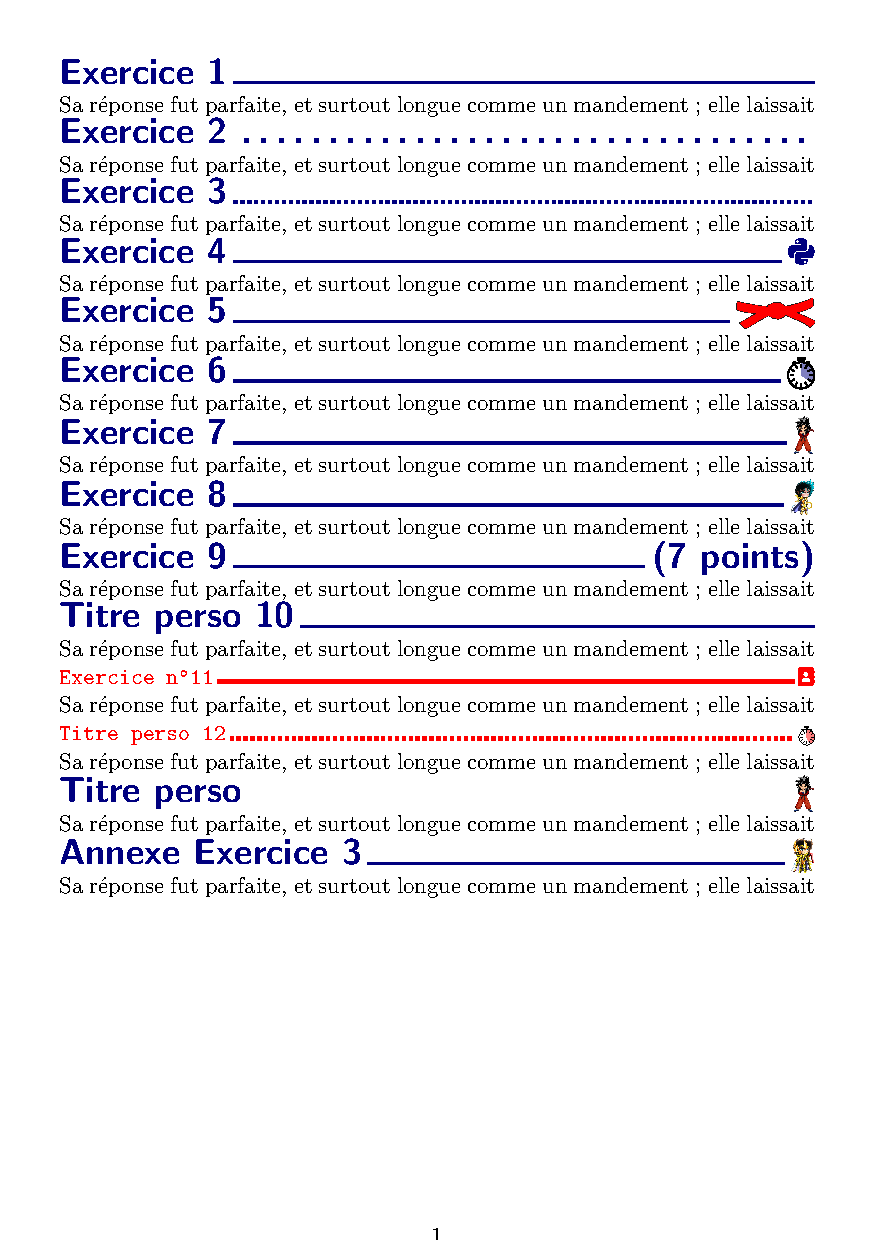
\includegraphics{envtexo_exemples.pdf}
\end{DemoCode}

\end{document}